\chapter{Le Gall Probability}

In this chapter I will cover the proofs, problems, and etc that are left to the reader. I will also add some remarks as I read through the text. I will also add some theorems and their proofs that are hard to understand in the text but I have made some helpful remarks.


\begin{problem}
	We define the discrete conditioning as
	\[ \prob'(A) = \prob(A|B) := \frac{\prob(A\cap B)}{\prob(B)} \]
	where $ A,B \in \mathcal{F} $ are measurable sets. Furthermore, we define the conditional expectation of a non-negative, or $ L^1 $ random variable $ X $ as
	\[ \E{X|B} := \frac{\E{\mathds{1}_B X}}{\prob(X)}. \]
	Show that $ \E{X|B} = \mathbb{E}_{\prob'}\left[X\right] $.
\end{problem}
\begin{solution}
	We first show this for a random variable given as
	\[ X = \alpha\mathds{1}_{B} \]
	for some $ A \in \mathcal{F} $. Observe that
	\begin{align*}
		\mathbb{E}_{\prob'}\left[X\right] &= \mathbb{E}_{\prob'}\left[\alpha \mathds{1}_A \right] = \alpha \mathbb{E}_{\prob'}\left[\mathds{1}_A\right] \\
		&= \alpha \prob'(A) = \alpha \prob(A|B) \\
		&= \alpha\frac{\prob(A\cap B)}{\prob(B)} \\
		&= \alpha \frac{\E{\mathds{1}_A\mathds{1}_B}}{\prob(B)} \\
		&= \frac{\E{\alpha \mathds{1}_A \mathds{1}_B}}{\prob(B)} \\
		&= \frac{\E{X\mathds{1}_B}}{\prob(B)} = \E{X|B}.
	\end{align*} 
	Using the linearity of the expectation, the conclusion above also follows for a simple random variable $ X = \sum_{i=1}^{n} \alpha_i \mathds{1}_{B_i} $ for $ B_i \in \mathcal{F} $ for all $ i=1,\dots,n $. Let $ X $ be a non-negative random variable. We can construct a sequence of random variables $ \set{X_n} $ such that $ X_n \uparrow X $. From monotone convergence theorem we have $ \mathbb{E}_{\prob'}\left[X_n \right] \uparrow \mathbb{E}_{\prob'}\left[X \right] $, as well as $ \E{\mathds{1}_B X_n} \uparrow \E{\mathds{1}_B X} $ as $ n\to\infty $. Since each $ X_n $ is a simple random variable we also have
	\[ \mathbb{E}_{\prob'}\left[X_n \right] = \frac{\E{X_n\mathds{1}_B}}{\prob(B)}. \]
	Letting $ n\to\infty $ on both sides of the equation above we will have
	\[ \mathbb{E}_{\prob'}\left[X \right] = \frac{\E{X\mathds{1}_B}}{\prob(B)}. \]
	And finally for the case that $ X \in L^1 $ we can write $ X = X^+ - X^- $ where $ X^+ $ and $ X^- $ are non-negative random variables and using the linearity of expectation it also follows that 
	\[ \mathbb{E}_{\prob'}\left[X \right] = \frac{\E{X\mathds{1}_B}}{\prob(B)}. \]
\end{solution}

\begin{definition}
	\label{def:E[X|Y]}
	Let $ X\in L^1(\Omega,\mathcal{A},\prob) $ be a random variable and $ Y: (\Omega,\mathcal{A}) \to (E,2^E) $ be a random variable that assumes its values in a countable set $ E $. The conditional expectation of $ X $ knowing $ Y $ is defined as
	\[ \E{X|Y} = \phi (Y), \]
	where $ \phi: E \to \R $ is given as
	\[ \phi(y) = \begin{cases}
		\E{X|Y=y} \quad & y\in E'\\
		0 \quad 		& y \notin E'
	\end{cases}, \]
	where $ E' = \set{y \in E: \prob(Y=y)> 0} $.
	
	\textbf{Alternatively}, let $ B_n = \inv{Y}(n) $ for $ n \in Y $. Then $ \mathcal{B} = \set{B_n}_{n\in E} $ is a countable partition for $ \Omega $. Let $ \mathcal{B} \supset \mathcal{B}' = \set{B \in \mathcal{B}: \prob(B) > 0}  $, i.e. those sets in the partition that has value zero. Then the conditional expectation of $ X $ knowing $ Y $ is given as
	\[ \E{X|Y} = \sum_{B \in \mathcal{B}'} \E{X|B}\mathds{1}_B. \]
	where $ \E{X|B} = \E{X\mathds{1}_B}/\prob(B) $ is as defined in Le Gall, page 228, first section of the page. Observe that with this definition it automatically follows that $ X = 0 $ on any $ B \notin \mathcal{B}' $.
\end{definition}
\begin{remark} 
	Note that the value of $ \phi(y) $ when $ y\not\in E' $ can be any number and this will change $ \E{X|Y} $ only on a set of measure zero. But it is convention to set it to be zero.
\end{remark}


\begin{theorem}
	Let $ Y: (\Omega,\mathcal{A}) \to (E,2^E) $ be a random variable where $ E $ is a countable set. Let $ X \in L^1(\Omega, \mathcal{A},\prob) $. Then we have $ \E{\abs{\E{X|Y}}} \leq \E{\abs{X}} $, and thus 
	\[ \E{X|Y} \in L^1(\Omega, \mathcal{A},\prob). \]
	Furthermore, for every bounded $ \sigma(Y) $-measurable random variable $ Z $ we have
	\[ \E{ZX} = \E{Z\E{X|Y}}. \]
\end{theorem}
\begin{proof}
	\textbf{Proof for $ \E{X|Y} \in L^1(\Omega,\mathcal{A},\prob) $:} 
	I will provide two proves for this. The first one is an elaborated version of Le Gall's proof, and the second one is my proof based on the stuff you can read in the appendix of this note.
	\begin{itemize}
		\item \textbf{Proof (1)} For Le Gall's proof we we will have
		\[ \E{\abs{\E{X|Y}}} = \sum_{y\in E'} \prob(Y=y)\abs{\E{X|Y=y}}. \]
		Note that for this step we used the definition of expectation for a random variable that takes countably many values (i.e. $ \E{X|Y} $). Note that since $ Y $ takes countably many values, then by the definition of $ \E{X|Y} $ (see Le Gall Definition 11.1), $ \E{X|Y} $ also assumes countably many values. Furthermore, note that $ E' = \set{y \in E: \prob(Y=y)> 0} $. A different way to write this is to use the partition generated by $ Y $. I.e. we can write
		\[ \E{\abs{\E{X|Y}}} = \sum_{B\in \mathcal{B}'} \prob(B) \abs{\E{X|B}} \]
		which is exactly the same as the first expression replacing $ \set{Y = y} $ with $ B $ and changing the summation index accordingly. So we will have
		\begin{align*}
			\E{\abs{\E{X|Y}}} &= \sum_{y\in E'} \prob(Y=y) \abs{\E{X|Y=y}} \\
			&= \sum_{y\in E'} \prob(Y=y) \abs{\frac{\E{X\mathds{1}_{\set{Y=y}}}}{\prob(Y=y)}} \\
			&= \sum_{y \in E'}\abs{\E{X\mathds{1}_{\set{Y=y}}}} \\
			&\leq \sum_{y\in E'}\E{\abs{X}\mathds{1}_{Y=y}} \\
			&= \E{\abs{X}\sum_{y\in E'}\mathds{1}_{\set{Y=y}}} \\
			&= \E{\abs{X}}.
		\end{align*}
		
		\item \textbf{Proof (2)}
		For this proof we will use the fact that since $ \E{X|Y} $ is $ \sigma(Y) $-measurable, then we can write it as
		\[ \E{X|Y} = \sum_{y\in E'} \E{X|Y=y} \mathds{1}_{Y=y} \]
		or equivalently
		\[ \E{X|Y} = \sum_{B\in \mathds{B}'} \E{X|B} \mathds{1}_{B}, \]
		where $ E' $ and $ \mathcal{B}' $ are as in \autoref{def:E[X|Y]}. For simplicity for the notation we will write $ \alpha_B = \E{X|B} $.
		
		So we will have
		\begin{align*}
			\E{\abs{\E{X|Y}}} &= \E{\abs{\sum_{B\in\mathcal{B}'} \alpha_B \mathds{1}_B }} \\
			&\leq \E{\sum_{B\in\mathcal{B}'}\abs{\alpha_B} \mathds{1}_B} \\
			&=\sum_{B\in\mathcal{B}'} \E{\abs{\alpha_B}\mathds{1}_B} \\
			&=\sum_{B\in\mathcal{B}'} \abs{\alpha_B} \prob(B) \\
			&=\sum_{B\in\mathcal{B}'} \frac{\abs{\E{X\mathds{1}_B}}}{\prob(B)}\prob(B) \\
			&\leq \sum_{B\in\mathcal{B}'} \E{\abs{X}\mathds{1}_B} \\
			&=\E{\abs{X}\sum_{B\in\mathcal{B}'}\mathds{1}_B} \\
			&=\E{\abs{X}}.
		\end{align*}
	\end{itemize}
	
	\noindent \textbf{Proof for $ \E{ZX} = \E{Z\E{X|Y}} $}. Since $ Z $ is $ \sigma(Y) $-measurable, by Proposition 8.9 Le Gall, we can find a bounded function $ \phi $ such that $ Z = \phi(Y) $. So we can write
	\begin{align*}
		\E{Z\E{X|Y}} &= \E{\phi(Y)\E{X|Y}} \\
		&= \sum_{y\in E} \phi(y) \E{X|Y=y}\prob(Y=y) \\
		&= \sum_{y\in E} \phi(y) \E{X\mathds{1}_{\set{Y=y}}}\\
		&= \E{X \sum_{y\in E} \phi(y) \mathds{1}_{\set{Y=y}} } \\
		&=\E{XZ},
	\end{align*}
	where we have used the Fubini's theorem to interchange $ \mathbb{E}  $ with sum, and also we used the fact that $ Z = \sum_{y\in E} \phi(y)\mathds{1}_{Y=y} $ (that follows from $ Z=\phi(Y) $).

\end{proof}


\begin{problem}
	In the properties of conditional expectation of random variables in Le Gall (page 234-245), right after part (d) he concludes that using the property (d) for any non-negative random variable $ (Y_n)_{n\in \N} $ we have
	\[ \E{\sum_n Y_n \big| \mathcal{B}} = \sum_n \E{Y_n|\mathcal{B}}. \]
	Prove this!
\end{problem}
\begin{solution}
	Since $ (Y_n)_{n\in \N} $ is non-negative, then the sequence of partial sums form an increasing sequence $\sum_{n=1}^{m}Y_n  = X_m\uparrow \sum_n Y_n $. Using the linearity of conditional expectation we can write
	\[ \E{\sum_{n=1}^{m} Y_n \big| \mathcal{B}} = \sum_{n=1}^{m} \E{Y_n \big| \mathcal{B}}. \]
	Taking the limit of both sides and using the property (d) we will have
	\[ \E{\sum_n Y_n \big| \mathcal{B}} = \sum_n \E{Y_n | \mathcal{B}}. \]
\end{solution}


\begin{proposition}[Properties of conditional expectation for integrable random variables]
	Let $ X \in L^1(\Omega,\mathcal{A},\prob) $. Then we have
	\begin{enumerate}[(a)]
		\item If $ X $ is $ \mathcal{B} $-measurable, then $ \E{X|\mathcal{B}} = X $.
		\item The mapping $ X\mapsto \E{X|\mathcal{B}} $ is linear on $ L^1(\Omega,\mathcal{A},\prob) $.
		\item If $ X\in L^1(\Omega,\mathcal{A},\prob) $, then $ \E{\E{X|\mathcal{B}}} = \E{X} $.
		\item If $ X\in L^1(\Omega,\mathcal{A},\prob) $, then $ \abs{\E{X|\mathcal{B}}} \leq \E{\abs{X}|\mathcal{B}} $ a.s. and consequently, we have
		\[ \E{\abs{\E{X|\mathcal{B}}}} \leq \E{\abs{X}}. \]
		There for the mapping $ X \mapsto \E{X|\mathcal{B}} $ is a contraction mapping of $ L^1(\Omega, \mathcal{A},\prob) $.
		\item Let $ X,X'\in L^1(\Omega,\mathcal{A},\prob) $ where $ X\geq X' $. Then it implies that 
		\[ \E{X|B} \geq \E{X'|\mathcal{B}}. \]
	\end{enumerate}
\end{proposition}
\begin{proof}
	\begin{enumerate}[(a)]
		\item By definition of conditional expectation for integrable random variables (see Theorem and Definition 11.3 Le Gall) the conditional expectation of $ X $ is a unique (up to a set of measure zero) $ \mathcal{B} $-measurable random variable. On the other hand $ X $ is itself a $ \mathcal{B} $-measurable random variable. So $ \E{X|\mathcal{B}} = B $ almost surely.
		\item Let $ X,X' $ be two random variables and $ \alpha,\beta \in \R $. Then for all random variable $ Z $ that is $ \mathcal{B} $-measurable we have
		\[ \E{Z(\alpha X + \beta X')} = \E{Z\E{\alpha X + \beta X'|\mathcal{B}}}. \]
		Using the linearity of expectation, as well as the characterization of conditional expectation (11.1 Le Gall), for the LHS we have
		\begin{align*}
			\E{Z(\alpha X + \beta X')} = \alpha\E{ZX} + \beta\E{ZX'} &= \alpha\E{Z\E{X|\mathcal{B}}} + \beta\E{Z\E{X'|\mathcal{B}}} \\
			&= \E{Z(\alpha\E{X|\mathcal{B}}+\beta\E{X'|\mathcal{B}})}.
		\end{align*}
		Thus we have
		\[ \E{Z\E{\alpha X + \beta X'|\mathcal{B}}} = \E{Z(\alpha\E{X|\mathcal{B}}+\beta\E{X'|\mathcal{B}})}. \]
		This implies
		\[ \E{\alpha X + \beta X'|\mathcal{B}} = \alpha\E{X|\mathcal{B}} + \beta\E{X'|\mathcal{B}} \qquad a.s. \]
		
		\item Observe that constant random variable $ X\equiv 1 $ is a $ \mathcal{B} $-measurable random variable. Using the characterization (11.2 Le Gall) it implies that  
		\[ \E{X} = \E{\E{X|\mathcal{B}}}. \]
		Equivalently, we can use the characterization (11.1 Le Gall) where we take $ B = \Omega $. Thus
		\[ \E{X} = \E{\mathds{1}_\Omega X} = \E{\mathds{1}_\Omega\E{X|\mathcal{B}}} = \E{\E{X|\mathcal{B}}}. \]
		
		\item First, observe that for any random variable $ X\geq 0 $ implies $ \E{X|\mathcal{B}} \geq 0 $. For $ X\in L^(\Omega,\mathcal{A},\prob) $ we can write
		\[ X = X^+ - X^-. \]
		Thus we can write
		\[ \abs{\E{X|\mathcal{B}}} = \abs{\E{X^+|\mathcal{B}} + \E{X^-|\mathcal{B}}} \leq \abs{\E{X^+|\mathcal{B}}} + \abs{\E{X^-|\mathcal{B}}} = \E{X^+|\mathcal{B}} + \E{X^-|\mathcal{B}} = \E{\abs{X}|\mathcal{B}}. \]
		The second part (the mapping being a contraction) follows immediately
		\[  \norm{\E{X|\mathcal{B}}}_1 = \E{\abs{\E{X|\mathcal{B}}}} \leq \E{\E{\abs{X}|\mathcal{B}}} = \E{\abs{X}} = \norm{X}.  \]
		
		\item We again use the fact that $ X\geq 0 $ implies $ \E{X|\mathcal{B}}>0 $ (see Lemma below for the proof). The using the linearity of conditional expectation we have
		\[ 0 \leq \E{(X-X')|\mathcal{B}} = \E{X|\mathcal{B}} - \E{X'|\mathcal{B}}. \]
		This implies that
		\[ \E{X|\mathcal{B}}\geq \E{X'|\mathcal{B}}. \]
	\end{enumerate}
\end{proof}

In the proof above, we used the fact $ X\geq 0 $ implies $ \E{X|\mathcal{B}}\geq 0 $. We prove this fact in the following Lemma.
\begin{lemma}
	Let $ X\geq 0 $ be in $ L^1(\Omega,\mathcal{A},\prob) $, and $ \mathcal{B} $ any sub $\sigma\text{-algebra}$. Then $ \E{X|\mathcal{B}}  \geq 0 $ almost surely.
\end{lemma}
\begin{proof}
	We simply use the characterization (11.1 Le Gall). Let $ B \in \mathcal{B} $. Then
	\[ \E{\mathds{1}_B X} = \mathcal{\mathds{1}_B \E{X|\mathcal{B}}}. \]
	We know the LHS is non-negative for all $ B\in \mathcal{[B]} $. This implies
	\[ \E{\mathcal{\mathds{1}_B \E{X|\mathcal{B}}}} \geq 0, \quad \forall B \in \mathcal{B}. \]
	Then it implies that
	\[ \E{X|\mathcal{B}} \geq 0. \]
\end{proof}

\begin{summary}[Conditional expectation]
	Le Gall starts developing the theory of conditional expectation by first considering the discrete conditioning. Then he generalizes it to conditioning with respect to some $\sigma\text{-algebra}$ where the theory is developed for $ L^1 $ functions. Finally, he derives the notion of conditional expectation generally for any non-negative random variable that can be unbounded and even not integrable. However, for general random variables, we need the condition of integrablity $ L^1 $ to make the reasoning above for $ X^+ $ and $ X^- $ separately.
\end{summary}

\begin{proposition}
	Let $ X,Y $ be real random variable and assume that $ Y $ is $ \mathcal{B} $-measurable. Then
	\[ \E{YX|\mathcal{B}} = Y \E{X|\mathcal{B}} \]
	provided $ X $ and $ Y $ are both non-negative or $ X $ and $ XY $ are both integrable.
\end{proposition}
\begin{proof}
	First we assume that $ X,Y $ are both non-negative. Then using the characterization conditional expectation for non-negative random variables (see 11.3 Le Gall), for any $ Z $ a $ \mathcal{B} $-measurable random variable we can write
	\[ \E{Z \E{XY|\mathcal{B}}} = \E{XYZ} = \E{(ZY) X} = \E{ZY\E{X|\mathcal{B}}}, \]
	where we used the fact that $ YZ $ is $ \mathcal{B} $-measurable (since both of them are $ \mathcal{B} $-measurable). Again using the characterization of conditional expectation for non-negative random variables (11.3 Le Gall) we can write
	\[ \E{XY|\mathcal{B}} = Y \E{X|\mathcal{B}}. \]
	
	Now it remains to show this for the case when $ X $  and $ XY $ are both integrable random variables (i.e. are $ L^1 $). Then we can have the same argument as above for $ X = X^+ - X^- $ as well as $ Y = Y^+ - Y^- $. 
\end{proof}


\begin{summary}[Some notes on independent events]
	Let $ A \in \mathcal{A} $ be an event. We can depict this event as the following Venn diagram.
	\begin{center}
		\tikzset{every picture/.style={line width=0.75pt}} %set default line width to 0.75pt        
		
		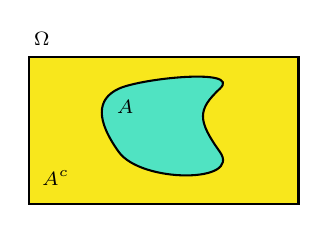
\begin{tikzpicture}[x=0.75pt,y=0.75pt,yscale=-1,xscale=1]
			%uncomment if require: \path (0,300); %set diagram left start at 0, and has height of 300
			
			%Shape: Rectangle [id:dp012872561340008914] 
			\draw  [fill={rgb, 255:red, 248; green, 231; blue, 28 }  ,fill opacity=1 ] (70,39.14) -- (200,39.14) -- (200,110) -- (70,110) -- cycle ;
			%Shape: Polygon Curved [id:ds13879352912763498] 
			\draw  [fill={rgb, 255:red, 80; green, 227; blue, 194 }  ,fill opacity=1 ] (113.33,54.32) .. controls (124.17,49.26) and (172.92,44.2) .. (162.08,54.32) .. controls (151.25,64.44) and (151.25,69.51) .. (162.08,84.69) .. controls (172.92,99.88) and (124.17,99.88) .. (113.33,84.69) .. controls (102.5,69.51) and (102.5,59.38) .. (113.33,54.32) -- cycle ;
			
			% Text Node
			\draw (111,58.4) node [anchor=north west][inner sep=0.75pt]  [font=\scriptsize]  {$A$};
			% Text Node
			\draw (75,92.4) node [anchor=north west][inner sep=0.75pt]  [font=\scriptsize]  {$A^{c}$};
			% Text Node
			\draw (71,25.4) node [anchor=north west][inner sep=0.75pt]  [font=\scriptsize]  {$\Omega $};
		\end{tikzpicture}
	\end{center}
	Let $ B \in \mathcal{A} $ with $ \prob(B) = p $. Then $ B $ is independent of $ A $ if and only if $ B $ occupies $ p $ proportion of $ A $ and its complement $ A^c $. I.e. the part of $ B $ that is in $ A $ should have $ \prob(A\cap B) = p \prob(A) $ and the portion of $ B $ that is in $ A^c $ should also have $ \prob(A^c\cap B) = p \prob(A^c) $ (this is literally the definition of independence). For instance, if $ \prob(B) = 0.2 $, then $ B $ should be such that occupies $ 20\% $  of $ A $ and $ 20\% $ of $ A^c $. A possible Venn diagram is
	\begin{center}
		
		
		\tikzset{every picture/.style={line width=0.75pt}} %set default line width to 0.75pt        
		
		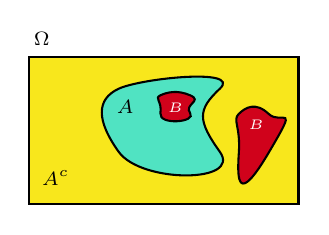
\begin{tikzpicture}[x=0.75pt,y=0.75pt,yscale=-1,xscale=1]
			%uncomment if require: \path (0,300); %set diagram left start at 0, and has height of 300
			
			%Shape: Rectangle [id:dp012872561340008914] 
			\draw  [fill={rgb, 255:red, 248; green, 231; blue, 28 }  ,fill opacity=1 ] (70,39.14) -- (200,39.14) -- (200,110) -- (70,110) -- cycle ;
			%Shape: Polygon Curved [id:ds13879352912763498] 
			\draw  [fill={rgb, 255:red, 80; green, 227; blue, 194 }  ,fill opacity=1 ] (113.33,54.32) .. controls (124.17,49.26) and (172.92,44.2) .. (162.08,54.32) .. controls (151.25,64.44) and (151.25,69.51) .. (162.08,84.69) .. controls (172.92,99.88) and (124.17,99.88) .. (113.33,84.69) .. controls (102.5,69.51) and (102.5,59.38) .. (113.33,54.32) -- cycle ;
			%Shape: Regular Polygon [id:dp15196214672803077] 
			\draw  [fill={rgb, 255:red, 208; green, 2; blue, 27 }  ,fill opacity=1 ] (133.45,57.48) .. controls (136.64,56.04) and (141.5,54.74) .. (147.79,57.48) .. controls (154.08,60.21) and (144.6,61.8) .. (147.79,66.11) .. controls (150.98,70.43) and (132.58,72.09) .. (133.45,66.11) .. controls (134.33,60.14) and (130.27,58.92) .. (133.45,57.48) -- cycle ;
			%Shape: Regular Polygon [id:dp8592034555506018] 
			\draw  [fill={rgb, 255:red, 208; green, 2; blue, 27 }  ,fill opacity=1 ] (171.24,66.42) .. controls (174.43,63.29) and (179.28,60.48) .. (185.58,66.42) .. controls (191.87,72.36) and (200.65,59.64) .. (185.58,85.19) .. controls (170.5,110.73) and (170.36,98.17) .. (171.24,85.19) .. controls (172.12,72.21) and (168.05,69.55) .. (171.24,66.42) -- cycle ;
			
			% Text Node
			\draw (111,58.4) node [anchor=north west][inner sep=0.75pt]  [font=\scriptsize]  {$A$};
			% Text Node
			\draw (75,92.4) node [anchor=north west][inner sep=0.75pt]  [font=\scriptsize]  {$A^{c}$};
			% Text Node
			\draw (71,25.4) node [anchor=north west][inner sep=0.75pt]  [font=\scriptsize]  {$\Omega $};
			% Text Node
			\draw (135.5,59.9) node [anchor=north west][inner sep=0.75pt]  [font=\tiny,color={rgb, 255:red, 255; green, 255; blue, 255 }  ,opacity=1 ]  {$B$};
			% Text Node
			\draw (174.5,67.9) node [anchor=north west][inner sep=0.75pt]  [font=\tiny,color={rgb, 255:red, 255; green, 255; blue, 255 }  ,opacity=1 ]  {$B$};
		\end{tikzpicture}
	\end{center}
	
\end{summary}

Now to understand the meaning of independent random variables we first need to understand the notion of independent $\sigma\text{-algebra}$s. Considering the summary above it is very easy to characterize this notion intuitively. Consider the following summary for more details.

\begin{summary}[Independence of $\sigma\text{-algebra}$s]
	The independence of two $\sigma\text{-algebra}$s is easiest to understand to understand when considering the atoms of $\sigma\text{-algebra}$s. One might argue that not all $\sigma\text{-algebra}$s will have such simple atoms. But the general philosophy of a theory in mathematics (for me at least) is to simply say ``\textbf{that} weird infinite dimensional and non imaginable object is (axiomatically) the same thing as \textbf{this} simple object that you can imagine and work with''. That is why we will provide only the intuitive explanation here and the whole theory that we will be developing will make sure that a similar kind of behaviour is also true for very complex situations that we are not even close the imagine them, let alone have arguments about them.
	
	Let $ \mathcal{B}_1 $ and $ \mathcal{B}_2 $ are two $\sigma\text{-algebra}$s with atoms $ \mathcal{A}_1 = \set{B_j} $ and $ \mathcal{A}_2 = \set{A_i} $. For instance, $ \mathcal{A}_2 $ can be depicted as below
	
	\begin{center}
		\tikzset{every picture/.style={line width=0.75pt}} %set default line width to 0.75pt        
		
		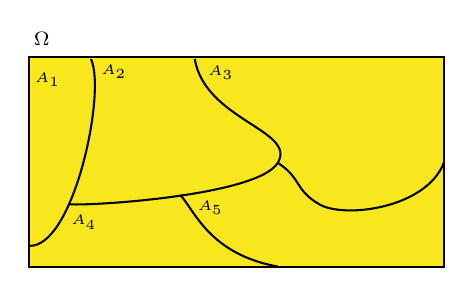
\begin{tikzpicture}[x=0.75pt,y=0.75pt,yscale=-1,xscale=1]
			%uncomment if require: \path (0,300); %set diagram left start at 0, and has height of 300
			
			%Shape: Rectangle [id:dp012872561340008914] 
			\draw  [fill={rgb, 255:red, 248; green, 231; blue, 28 }  ,fill opacity=1 ] (70,39.14) -- (270,39.14) -- (270,140) -- (70,140) -- cycle ;
			%Curve Lines [id:da3685683420702155] 
			\draw    (100,40) .. controls (107.5,56) and (91.5,131.5) .. (70,130) ;
			%Curve Lines [id:da09925164313047152] 
			\draw    (150,40) .. controls (155,69.5) and (199.37,74.31) .. (190,90) .. controls (180.63,105.69) and (101.27,110.79) .. (90,110) ;
			%Curve Lines [id:da9918813897008854] 
			\draw    (270,90) .. controls (261.5,112) and (222,117) .. (210,110) .. controls (198,103) and (201.5,97.5) .. (190,90) ;
			%Curve Lines [id:da08690554601759626] 
			\draw    (190,140) .. controls (157,134) and (150,113) .. (143,105.5) ;
			
			% Text Node
			\draw (71,25.4) node [anchor=north west][inner sep=0.75pt]  [font=\scriptsize]  {$\Omega $};
			% Text Node
			\draw (71.5,45.4) node [anchor=north west][inner sep=0.75pt]  [font=\tiny]  {$A_{1}$};
			% Text Node
			\draw (103.5,41.4) node [anchor=north west][inner sep=0.75pt]  [font=\tiny]  {$A_{2}$};
			% Text Node
			\draw (155,41.9) node [anchor=north west][inner sep=0.75pt]  [font=\tiny]  {$A_{3}$};
			% Text Node
			\draw (89,113.9) node [anchor=north west][inner sep=0.75pt]  [font=\tiny]  {$A_{4}$};
			% Text Node
			\draw (150,106.9) node [anchor=north west][inner sep=0.75pt]  [font=\tiny]  {$A_{5}$};
			
		\end{tikzpicture}
	\end{center}
	\FloatBarrier
	
	Then $ \mathcal{B}_1 $ is independent of $ \mathcal{B}_2 $ if every atom of $ \mathcal{B}_1 $ occupies the $ \prob(B_i) $ proportion of each $ A_i $. For instance if $ \prob(B_1) = 0.3 $ then $ \prob(B_1\cap A_i) = 0.3 \prob(A_i)$ for all $ A_i $. For instance we can depict this as the follows.
	
	\begin{center}
		\tikzset{every picture/.style={line width=0.75pt}} %set default line width to 0.75pt        
		
		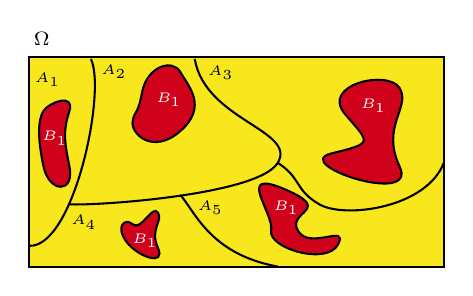
\begin{tikzpicture}[x=0.75pt,y=0.75pt,yscale=-1,xscale=1]
			%uncomment if require: \path (0,300); %set diagram left start at 0, and has height of 300
			
			%Shape: Rectangle [id:dp012872561340008914] 
			\draw  [fill={rgb, 255:red, 248; green, 231; blue, 28 }  ,fill opacity=1 ] (70,39.14) -- (270,39.14) -- (270,140) -- (70,140) -- cycle ;
			%Curve Lines [id:da3685683420702155] 
			\draw    (100,40) .. controls (107.5,56) and (91.5,131.5) .. (70,130) ;
			%Curve Lines [id:da09925164313047152] 
			\draw    (150,40) .. controls (155,69.5) and (199.37,74.31) .. (190,90) .. controls (180.63,105.69) and (101.27,110.79) .. (90,110) ;
			%Curve Lines [id:da9918813897008854] 
			\draw    (270,90) .. controls (261.5,112) and (222,117) .. (210,110) .. controls (198,103) and (201.5,97.5) .. (190,90) ;
			%Curve Lines [id:da08690554601759626] 
			\draw    (190,140) .. controls (157,134) and (150,113) .. (143,105.5) ;
			%Shape: Regular Polygon [id:dp11357503770338861] 
			\draw  [fill={rgb, 255:red, 208; green, 2; blue, 27 }  ,fill opacity=1 ] (77.09,65.1) .. controls (79.87,60.68) and (92.38,56.27) .. (89.6,65.1) .. controls (86.82,73.94) and (86.82,78.35) .. (89.6,91.61) .. controls (92.38,104.86) and (79.87,104.86) .. (77.09,91.61) .. controls (74.3,78.35) and (74.3,69.52) .. (77.09,65.1) -- cycle ;
			%Shape: Regular Polygon [id:dp22801095225143042] 
			\draw  [fill={rgb, 255:red, 208; green, 2; blue, 27 }  ,fill opacity=1 ] (124.69,55.78) .. controls (126.99,43.74) and (139.19,39.5) .. (143.1,46.34) .. controls (147.01,53.19) and (156.45,62.86) .. (143.1,74.67) .. controls (129.75,86.47) and (118.93,75.85) .. (120.08,69.95) .. controls (121.23,64.04) and (122.39,67.82) .. (124.69,55.78) -- cycle ;
			%Shape: Regular Polygon [id:dp08574179085383848] 
			\draw  [fill={rgb, 255:red, 208; green, 2; blue, 27 }  ,fill opacity=1 ] (120.16,119.63) .. controls (124.24,123.02) and (129.68,109.87) .. (132.25,113.97) .. controls (134.82,118.07) and (128.17,121.75) .. (132.25,130.94) .. controls (136.34,140.14) and (122.58,135.33) .. (117.13,128.11) .. controls (111.69,120.9) and (116.08,116.23) .. (120.16,119.63) -- cycle ;
			%Shape: Regular Polygon [id:dp5027282268067348] 
			\draw  [fill={rgb, 255:red, 208; green, 2; blue, 27 }  ,fill opacity=1 ] (222.44,66.59) .. controls (210.29,52.41) and (243.12,44.85) .. (248.7,53.99) .. controls (254.28,63.12) and (239.51,72.26) .. (248.7,91.79) .. controls (257.89,111.32) and (195.52,90.53) .. (215.87,85.49) .. controls (236.23,80.45) and (234.58,80.76) .. (222.44,66.59) -- cycle ;
			%Shape: Regular Polygon [id:dp6413319901261554] 
			\draw  [fill={rgb, 255:red, 208; green, 2; blue, 27 }  ,fill opacity=1 ] (193.25,102.7) .. controls (217.42,113.03) and (194.21,113.03) .. (199.69,122.69) .. controls (205.17,132.34) and (224.51,119.02) .. (219.03,129.35) .. controls (213.55,139.67) and (185.19,131.01) .. (186.8,122.69) .. controls (188.41,114.36) and (169.07,92.38) .. (193.25,102.7) -- cycle ;
			
			% Text Node
			\draw (71,25.4) node [anchor=north west][inner sep=0.75pt]  [font=\scriptsize]  {$\Omega $};
			% Text Node
			\draw (71.5,45.4) node [anchor=north west][inner sep=0.75pt]  [font=\tiny]  {$A_{1}$};
			% Text Node
			\draw (103.5,41.4) node [anchor=north west][inner sep=0.75pt]  [font=\tiny]  {$A_{2}$};
			% Text Node
			\draw (155,41.9) node [anchor=north west][inner sep=0.75pt]  [font=\tiny]  {$A_{3}$};
			% Text Node
			\draw (89,113.9) node [anchor=north west][inner sep=0.75pt]  [font=\tiny]  {$A_{4}$};
			% Text Node
			\draw (150,106.9) node [anchor=north west][inner sep=0.75pt]  [font=\tiny]  {$A_{5}$};
			% Text Node
			\draw (75,73.4) node [anchor=north west][inner sep=0.75pt]  [font=\tiny,color={rgb, 255:red, 255; green, 255; blue, 255 }  ,opacity=1 ]  {$B_{1}$};
			% Text Node
			\draw (130,54.9) node [anchor=north west][inner sep=0.75pt]  [font=\tiny,color={rgb, 255:red, 255; green, 255; blue, 255 }  ,opacity=1 ]  {$B_{1}$};
			% Text Node
			\draw (228.5,57.9) node [anchor=north west][inner sep=0.75pt]  [font=\tiny,color={rgb, 255:red, 255; green, 255; blue, 255 }  ,opacity=1 ]  {$B_{1}$};
			% Text Node
			\draw (186.5,106.9) node [anchor=north west][inner sep=0.75pt]  [font=\tiny,color={rgb, 255:red, 255; green, 255; blue, 255 }  ,opacity=1 ]  {$B_{1}$};
			% Text Node
			\draw (118.5,122.9) node [anchor=north west][inner sep=0.75pt]  [font=\tiny,color={rgb, 255:red, 255; green, 255; blue, 255 }  ,opacity=1 ]  {$B_{1}$};
		\end{tikzpicture}
	\end{center}
	\FloatBarrier
	Another way to write this is for every $ B \in \mathcal{B}_1 $ to have
	\[ \E{\mathds{1}_B| \mathcal{B}_2} = \prob(B). \]
	And we say that two random variables $ X,Y $ are independent, if their generating $\sigma\text{-algebra}$s are independent. For example, let $ d_n $ and $ d_m $ be two dyadic functions. If $ n\neq m $ then $ d_n $ and $ d_m $ are independent.
	\begin{center}
		
		
		\tikzset{every picture/.style={line width=0.75pt}} %set default line width to 0.75pt        
		
		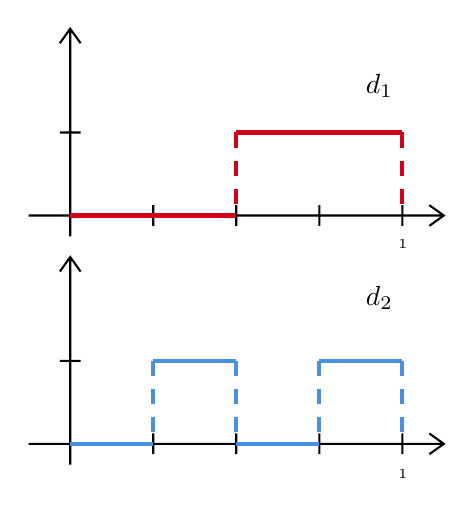
\begin{tikzpicture}[x=0.75pt,y=0.75pt,yscale=-1,xscale=1]
			%uncomment if require: \path (0,300); %set diagram left start at 0, and has height of 300
			
			%Shape: Axis 2D [id:dp9615379005807485] 
			\draw  (90,160) -- (290,160)(110,70) -- (110,170) (283,155) -- (290,160) -- (283,165) (105,77) -- (110,70) -- (115,77) (150,155) -- (150,165)(190,155) -- (190,165)(230,155) -- (230,165)(270,155) -- (270,165)(105,120) -- (115,120) ;
			\draw   ;
			%Straight Lines [id:da04897594804446026] 
			\draw [color={rgb, 255:red, 208; green, 2; blue, 27 }  ,draw opacity=1 ][line width=1.5]    (110,160) -- (190,160) ;
			%Straight Lines [id:da6204413266865749] 
			\draw [color={rgb, 255:red, 208; green, 2; blue, 27 }  ,draw opacity=1 ][line width=1.5]    (190,120) -- (270,120) ;
			%Straight Lines [id:da9803718824866479] 
			\draw [color={rgb, 255:red, 208; green, 2; blue, 27 }  ,draw opacity=1 ][line width=1.5]  [dash pattern={on 5.63pt off 4.5pt}]  (190,120) -- (190,160) ;
			%Straight Lines [id:da5963309319883598] 
			\draw [color={rgb, 255:red, 208; green, 2; blue, 27 }  ,draw opacity=1 ][line width=1.5]  [dash pattern={on 5.63pt off 4.5pt}]  (270,120) -- (270,160) ;
			%Shape: Axis 2D [id:dp8267116446963094] 
			\draw  (90,270) -- (290,270)(110,180) -- (110,280) (283,265) -- (290,270) -- (283,275) (105,187) -- (110,180) -- (115,187) (150,265) -- (150,275)(190,265) -- (190,275)(230,265) -- (230,275)(270,265) -- (270,275)(105,230) -- (115,230) ;
			\draw   ;
			%Straight Lines [id:da8499928443543412] 
			\draw [color={rgb, 255:red, 74; green, 144; blue, 226 }  ,draw opacity=1 ][fill={rgb, 255:red, 74; green, 144; blue, 226 }  ,fill opacity=1 ][line width=1.5]    (110,270) -- (150,270) ;
			%Straight Lines [id:da5467434321150186] 
			\draw [color={rgb, 255:red, 74; green, 144; blue, 226 }  ,draw opacity=1 ][fill={rgb, 255:red, 74; green, 144; blue, 226 }  ,fill opacity=1 ][line width=1.5]    (150,230) -- (190,230) ;
			%Straight Lines [id:da15502721097766203] 
			\draw [color={rgb, 255:red, 74; green, 144; blue, 226 }  ,draw opacity=1 ][fill={rgb, 255:red, 74; green, 144; blue, 226 }  ,fill opacity=1 ][line width=1.5]    (190,270) -- (230,270) ;
			%Straight Lines [id:da6979672326952524] 
			\draw [color={rgb, 255:red, 74; green, 144; blue, 226 }  ,draw opacity=1 ][fill={rgb, 255:red, 74; green, 144; blue, 226 }  ,fill opacity=1 ][line width=1.5]    (230,230) -- (270,230) ;
			%Straight Lines [id:da6829823450497226] 
			\draw [color={rgb, 255:red, 74; green, 144; blue, 226 }  ,draw opacity=1 ][line width=1.5]  [dash pattern={on 5.63pt off 4.5pt}]  (150,230) -- (150,270) ;
			%Straight Lines [id:da8114389723038795] 
			\draw [color={rgb, 255:red, 74; green, 144; blue, 226 }  ,draw opacity=1 ][line width=1.5]  [dash pattern={on 5.63pt off 4.5pt}]  (190,230) -- (190,270) ;
			%Straight Lines [id:da824558084081193] 
			\draw [color={rgb, 255:red, 74; green, 144; blue, 226 }  ,draw opacity=1 ][line width=1.5]  [dash pattern={on 5.63pt off 4.5pt}]  (230,230) -- (230,270) ;
			%Straight Lines [id:da465469102564559] 
			\draw [color={rgb, 255:red, 74; green, 144; blue, 226 }  ,draw opacity=1 ][line width=1.5]  [dash pattern={on 5.63pt off 4.5pt}]  (270,230) -- (270,270) ;
			
			% Text Node
			\draw (251,90.4) node [anchor=north west][inner sep=0.75pt]    {$d_{1}$};
			% Text Node
			\draw (251,192.4) node [anchor=north west][inner sep=0.75pt]    {$d_{2}$};
			% Text Node
			\draw (266.5,169.9) node [anchor=north west][inner sep=0.75pt]  [font=\tiny]  {$1$};
			% Text Node
			\draw (266.5,280.9) node [anchor=north west][inner sep=0.75pt]  [font=\tiny]  {$1$};
		\end{tikzpicture}
	\end{center}
	The atoms of the generated $\sigma\text{-algebra}$s by these random variables is
	\[ \mathcal{A}_1 = \set{(0,1/2],(1/2,1]},\qquad \mathcal{A}_2 = \set{(0,1/4]\cup (1/2,3/4], (1/4,1/2] \cup  (3/4,1]}. \]
	It is easy to check that the sets in these atoms are independent.
\end{summary}

\begin{example}
	Using the characterization of independent above, it is easy to prove some properties of conditional expectation (at least for discrete case where we can use the characterization above). Using this characterization prove that if $ \mathcal{B}_1 $ and $ \mathcal{B}_2 $ are two independent $\sigma\text{-algebra}$s, and if $ X $ is $ \mathcal{B}_1 $ measurable, then we have
	\[ \E{X|B_2} = \E{X}. \]
\end{example}
\begin{solution}
	Denote the atoms of $ \mathcal{B}_1 $ and $ \mathcal{B}_2 $ by $ \mathcal{A}_1 $ and $ \mathcal{A}_2 $ respectively. Then we can write $ X $ as 
	\[ X = \sum_{B \in \mathcal{A}_1} \alpha_i \mathds{1}_B.  \]
	So using the linearity of the conditional expectation we can write
	\[ \E{X|B_2} = \E{\sum_{B\in\mathcal{A}_1}\alpha_i \mathds{1}_B\big|B_2} = \sum_{B\in\mathcal{A}_1}\alpha_i \E{\mathds{1}_B|B_2} = \sum_{B\in\mathcal{A}_1} \alpha_i \prob(B) = \E{X}. \]
\end{solution}


\begin{proposition}
	Two sub-$\sigma\text{-algebra}$s $ \mathcal{B}_1 $ and $ \mathcal{B}_2 $ are independent if and only if for every $ B \in \mathcal{B}_2 $, we have $ \E{\mathds{1}_B|\mathcal{B}_2} = \prob(B) $.
\end{proposition}
\begin{proof}
	$ \boxed{\Rightarrow} $ We assume that $ \mathcal{B}_1 $ and $ \mathcal{B}_2 $ are independent (for the definition of independent $\sigma\text{-algebra}$s see Le Gall page 169). Let $ B \in \mathcal{B}_1 $ and $ Z $ any $ \mathcal{B}_2 $-measurable random variable. By characterization of conditional expectation  (11.3 Le Gall) we can write
	\begin{align*}
		\E{Z\E{\mathds{1}_B|\mathcal{B}_2}} &= \E{Z\mathds{1}_B} \\
		&= \E{Z}\E{\mathds{1}_B} && \text{(by independence of $ \mathds{1}_B $ and $ Z $)} \\
		&= \prob(B) \E{Z} \\
		&= \E{\prob(B)Z}. && \text{(linearity of expectation)}
	\end{align*}
	This implies that 
	\[ \E{\mathds{1}_B|\mathcal{B}_2} = \prob(B) \quad a.s. \]
	
	\noindent $ \boxed{\Leftarrow} $ Let $ B_1 \in \mathcal{B}_1 $ and $ B_2 \in \mathcal{B}_2 $. We want to show $ \prob(B_1\cap B_2) = \prob(B_1) \prob(B_2) $ or equivalently $ \E{\mathds{1}_{B_1} \mathds{1}_{B_2}} = \E{\mathds{1}_{B_1}} \E{\mathds{1}_{B_2}} $. To see this we can write
	\begin{align*}
		\E{\mathds{1}_{B_1} \mathds{1}_{B2}} &= \E{\mathds{1}_{B_1} \E{\mathds{1}_{B_2}|\mathcal{B}_1}}  && \text{(characterization of cond. expec.)} \\
		&=\E{\mathds{1}_{B_1} \prob(B_2)} && \text{(by assumption above)} \\
		&=\prob(B_2) \E{\mathds{1}_{B_1}} && \text{(by linearity of expec.)} \\
		&= \prob(B_2) \prob(B_1).
	\end{align*}
\end{proof}

\begin{proposition}
	If $ \mathcal{B}_1 $ and $ \mathcal{B}_2 $ are independent, we have $ \E{X|\mathcal{B}_1} = \E{X} $ for every non-negative $ \mathcal{B}_2 $-measurable random variable $ X $ and for every $ X \in L^1(\Omega,\mathcal{B}_2,\prob) $.
\end{proposition}
\begin{proof}
	Assume $ X $ is non-negative random variable that is $ \mathcal{B}_2 $-measurable. Let $ Z $ be a $ \mathcal{B}_1 $-measurable random variable. Then using the independence of $\sigma\text{-algebra}$s we can write
	\[ \E{XZ} = \E{X}\E{Z} = \E{\E{X} Z}. \]
	Thus this satisfies the characteristic property (11.3) and thus $ \E{X|\mathcal{B}_1} = \E{X} $. When $ X $ is $ L^1 $ then we can have the same argument for each negative and positive parts $ X = X^+ - X^- $.opol
\end{proof}